\chapter{Programmstruktur}

Abbildung \ref{B_UML} zeigt den prinzipiellen Programmaufbau per Klassendiagramm nach UML 2.4.1 \cite{W_UMLInfra}\cite{W_UMLSuper}.
Abgebildet sind die wichtigsten Klassen mit ihren grunds�tzlichen Beziehungen zueinander.
Auf Angabe der Attribute und Operationen wurde aus Platzgr�nden verzichtet.
Der Aufbau des Programms gliedert sich grunds�tzlich in zwei Teile:
zum einen die Klassen f�r die Ansteuerung, Eingabe und Ausgabe,
zum anderen die Generatorklassen plus generierte Objekte.

\emph{CEventReceiver} empf�ngt Inputs und leitet diese an die anderen Objekte weiter.
\emph{CGUI} definiert die Anordnung der GUI-Elemente.
\emph{COptionen} steuert die einzelnen Klassen an, zus�tzlich werden hier sowohl Einstellung als auch Ergebnisse geladen und gespeichert.
In dieser Klasse ist zugleich der Pipeline-Ablauf definiert.
\emph{CSzene} stellt sowohl die GUI als auch die Dungeonszene dar.
Hierzu sind Methoden vorhanden, um die Dungeonszene aus den einzelnen Teilen zusammenzusetzen.
Die \emph{main}-Klasse enth�lt neben Initialisierungen eine Programmschleife zum Betrieb der Irrlicht-Engine.

\emph{CFraktalGenerator} erstellt L-Systeme und deren Ableitungen, welche die Turtle-Grafik-Zeichenanweisungen darstellen.
\emph{CVoxelRaum} verwaltet den Voxelraum, zeichnet die Turtle-Grafik-Zeichenanweisungen und f�hrt Erosion sowie Filterung schwebender Fragmente durch.
\emph{CDreiecksMesh} verwaltet die H�hlensubnetze, f�hrt die Umwandlung Voxel zu Dreiecksnetz durch, berechnet Sichtbarkeitsinformationen 
der H�hle und f�hrt die Reduktion der H�hlensubnetze durch.
\emph{CArchitekt} verwaltet Vorlagen f�r R�ume, Detailobjekte sowie die Grundkonfiguration der G�nge
und konstruiert aus einer gegebenen Voxelh�hle durch das Platzieren von G�ngen und R�umen den Dungeon.
Bei der Erstellung von Andockstellen an der H�hle wird auf Vertexkoordinaten-Berechnungsroutinen von CDreiecksMesh zur�ckgegriffen.
Die R�ume \emph{SDungeonRaum} tragen einen Verweis auf die zugrundeliegende Subzene \emph{CSubSzene}, welche die Geometrie des Raums enth�lt.
Jeder Gang ist eine Instanz von \emph{CSpline}.
F�r deren Erstellung werden von CArchitekt aus Gangparameter,
ermittelte Andockstellen sowie Informationen aus Detailobjektvorlagen \emph{SSplineDetailobjektVorlage} an CSpline �bergeben.
Hier erfolgt die Generierung der Ganggeometrie und Adaptergeometrien sowie die Platzierung der Detailobjekte als \emph{SSplineDetailobjekt}.
Sichtbarkeitsinformationen der G�nge und Gangreduktionsstufen werden ebenfalls in CSpline berechnet.

Es existieren zwei separate Zufallsgeneratoren vom Typ \emph{CZufallsGenerator}:
einer ist f�r CDreiecksMesh zust�ndig und wird dort f�r das Verwackeln der Eckpunkte eingesetzt,
der andere liefert Zufallswerte f�r die restlichen Klassen.


%welche Verfahren wurden implementiert?
%-> besonders wichtig, falls Alternativen genannt wurden, wie z.B. beim Zeichnen von Strichen im Voxerkaum
%Bibliotheken
%- Irrlicht
%Coding-Konventionen:
%- eigene
%- Irrlicht: http://irrlicht.sourceforge.net/faq.html
%UML, Pap
%VoxelRaum:
%- direkter Zugriff auf das Voxel-Array statt LeseVoxel() 
%- MinVoxelRandOffset == 3:
%-> keine Spezialf�llen an R�ndern
%--> deutliche Beschleunigung (ca. Faktor 4-10, je nach Prozedur)
%- Eigene Irrlichklassen erl�utern
%OBJ-Format erkl�ren:
%- Irrlicht-Exporter
%- eigener Exporter
%Wichtig: Beim Durchlauf durch Voxelraum: (bezieht sich auf Visual Studio 2010, vermutlich bei den meisten anderen Compiler gleiche Ablage im Speicher)
%- Schleifen-Reihenfolge von aussen nach innen m�glichst immer X,Y,Z -> effektiverer Speicherzugriff (nacheinander folgende Elemente stehen auch nacheinander im Speicher) -> merkbar schneller


\begin{figure}[hbtp]
  \centering   % trim: links unten rechts oben
	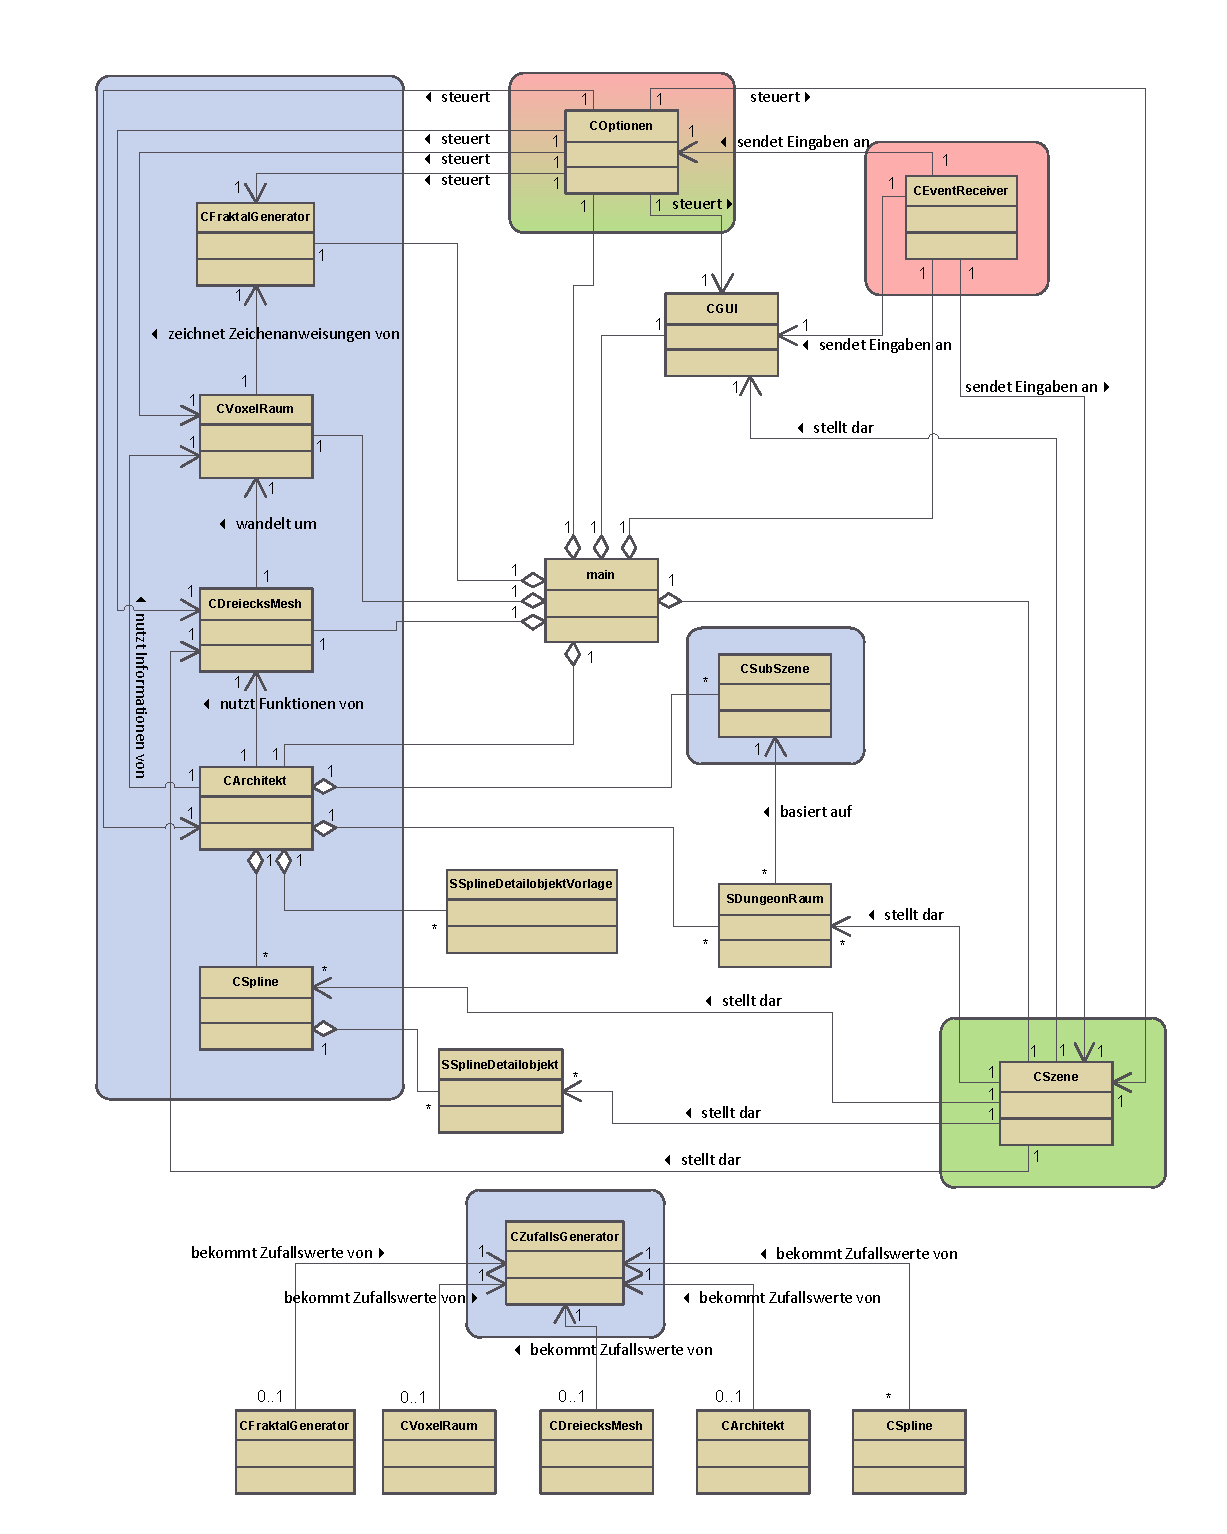
\includegraphics[width=15cm,trim = 10mm 6mm 6mm 10mm,clip]{Bilder/UML-DunGen}
	\caption[Programmaufbau - UML Klassendiagramm]{\emph{Programmaufbau - UML Klassendiagramm}:
	Dargestellt ist der prinzipielle Aufbau des Dungeongenerator-Programms.
	Auf die Darstellung von Klassen der Irrlicht-Engine wurde verzichtet.
	Der Inputteil ist \emph{rot} markiert, die eigentlichen Generatoren \emph{blau} und der Outputteil \emph{gr�n}.
	}
	\label{B_UML}
\end{figure}


\section{Anmerkung zum Rendering}

Die generierten Dreiecksnetze der H�hle sowie die der G�nge mit ihren Adaptern sind
bez�glich der Positionen ihrer Vertices bereits korrekt zueinander ausgerichtet.
Das bedeutet, dass sie untransformiert in den Szenegraphen eingebunden werden k�nnen.
Beim Rendering per Shader entfallen somit die Transformationen zur Berechnung der resultierenden Vertexpositionen und Normalen.
Es braucht nur die Projektionstransformation von 3D-Raumkoordinaten zu 2D-Bildschirmkoordinaten durchgef�hrt zu werden.
Durch das Weglassen der �brigen Transformationen ist eine h�here Performanz erzielbar.

%H�hlenmesh besitzt im allgemeinen viele Vertices und Dreiecke
%-> Falls im Shader Vertex-Positionen oder Vertex-Normalen benutzt werden:
%  - Mesh m�glichst untransformiert einbinden oder vorher transformieren (wenn statische Transformation)
%	-> keine Transformation im Shader n�tig -> spart Berechnungsaufwand
%- F�r Beleuchtung:
%  - im Normalfall reicht es aus die Lichtquelle zu transformieren, diese muss relativ zur H�hle korrekt positioniert und ausrichtet befinden
%  
%trifft auch f�r G�nge zu:
%alle vom Generator prozedural generierten Objekte brauchen keine Transformationen, sondern sind relativ zueinander korrekt positioniert und ausgerichtet
%
